% !TEX root = diss.tex

\chapter{Theory}
\label{ch:theory}

\section{The quantum mechanical approach}

The fundamental properties governing all of chemistry are dictated by the quantum mechanical wave functions, $\Psi$. Therefore, in quantum chemistry we seek solutions to the non-relativistic time-independent Schr{\"o}dinger equation
\begin{equation}
\hham \ket{\Psi} = E \ket{\Psi}
\label{eq:schrodinger}
\end{equation}

\noindent where $\hham$ is the Hamiltonian operator for a system of nuclei and electrons, and $\Psi$ is the wave function, defined as the set of eigenvectors with energy eigenvalues $E$.\cite{Griffiths2016} For a system with $N$ electrons and $M$ nuclei, the full Hamiltonian in atomic units is

\begin{equation}
\begin{split}
\hham = &-\sum_{i=1}^N \frac{1}{2}\nabla_i^2 - \sum_{A=1}^M\frac{1}{2M_A}\nabla_A^2
-\sum_{i=1}^M\sum_{A=1}^M\frac{Z_A}{r_{iA}} \\
&+ \sum_{i=1}^N\sum_{j>i}^N \frac{1}{r_{ij}} + \sum_{A=1}^M\sum_{B>A}^M
\frac{Z_A Z_B}{R_{AB}}
\label{eq:ham}
\end{split}
\end{equation}

\noindent In this equation, $Z_A$ is the atomic number of nucleus $A$ with a mass $M_A$ divided by the mass of an electron. The Laplacian operators $\nabla_i^2$ and $\nabla_A^2$ represent differentiation with respect to the coordinates of the $ith$ electron and $Ath$ nucleus. The first and second terms are the kinetic energies of the electrons and nuclei, respectively. The third term represents the Coulomb attraction between electrons and nuclei with distance $r_{iA}$. The fourth and fifth terms represent repulsion between two electrons with distance $r_{ij}$, and between two nuclei with distance $R_{AB}$, respectively.

Nuclei move slowly relative to electrons, due to their much greater mass. This is the central pillar of the Born-Oppenheimer approximation that is nearly always applied in molecular electronic structure calculations. The application of this approximation allows for the simplification of Equation~\ref{eq:ham}: using a separation of electronic an nuclear variables, the second term for nuclear kinetic energy is solved separately. Also, the last term of nuclear repulsion is constant, and thus is generally ignored. This leaves us with the electronic Hamiltonian

\begin{equation}
  \hham_{elec} = -\sum_{i=1}^N \frac{1}{2}\nabla_i^2  -\sum_{i=1}^M\sum_{A=1}^M\frac{Z_A}{r_{iA}}
  + \sum_{i=1}^N\sum_{j>i}^N \frac{1}{r_{ij}}
\label{eq:hamelect}
\end{equation}

\noindent Unfortunately, it is only possible to exactly solve the Schr{\"o}dinger equation for the full electronic Hamiltonian $\hham_{elec}$ in the simplest of cases: when there is only one electron (H, \ch{H_2^+}, \ch{He^+}, \ch{Li^{2+}}, etc). Note that since we will always work within the Born-Oppenheimer approximation, the subscript \emph{elec} is usually dropped.  In order to proceed to systems with multiple electrons, we must make further approximations.

\subsection{Spin and Spatial Orbitals}

We will refer to the wave function of a single particle as an orbital. Naturally then, as we will deal with electrons in molecules, we shall refer to their wave functions as molecular orbitals (MOs). To fully describe electrons we must consider a spatial and spin component to the overall wave function. A spatial orbital $\psi_i$(\textbf{r}), is a function of the position vector \textbf{r}, and describes the distribution of an electron in all space. It is usually assumed that spatial MOs form an orthonormal set such that

\begin{equation}
\bra{\psi_i(\mathbf{r})}\ket{\psi_j(\mathbf{r})} =
\int d\mathbf{r} \psi_i^*(\mathbf{r})\psi_j(\mathbf{r}) = \delta_{ij}
\label{eq:orthonormal}
\end{equation}

\noindent where the left-hand side is standard Dirac \emph{bra-ket} notation representing the same integral in the middle. The right-hand side of Equation~\ref{eq:orthonormal} is the standard Kronecker delta.

The spin of an electron is represented by two orthonormal functions $\alpha(\omega)$ and $\beta(\omega)$, or spin up and spin down. If a wave function describes both the spatial distribution and spin of an electron it is a spin orbital, $\chi_i(\mathbf{r})$, where \textbf{x} represents both the spatial distribution and spin coordination of an electron ($\mathbf{x} = \{ \mathbf{r}, \omega \}$). Since $\psi_i(\mathbf{r})$ and $\alpha(\omega)/\beta(\omega)$ are orthonormal, so too is $\chi_i(\mathbf{x})$

\begin{equation}
\bra{\chi_i(\mathbf{x})}\ket{\chi_j(\mathbf{x})} = \delta_{ij}
\end{equation}

\subsection{The Hartree product}

The first steps towards describing an $N$ electron wave function come from the work in the late 1920s by Hartree. The early \emph{Hartree method} took an approach in which the wave function of $N$ non-interacting electrons ($\Psi^{HP}$) is described by the product of $N$ spin orbitals, known as a \emph{Hartree product}:

\begin{equation}
\Psi^{HP}(\mathbf{x}_1,\mathbf{x}_2,\ldots,\mathbf{x}_N) = \chi_i(\mathbf{x}_1)\chi_j(\mathbf{x}_2)\dots\chi_k(\mathbf{x}_N)
\end{equation}

\noindent In such a system the Hamiltonian has the form of a sum of $N$ independent operators

\begin{equation}
  \hham = \sum_{i=1}^N \hat{h}(i)
\end{equation}

\noindent where $\hat{h}(i)$ is

\begin{equation}
  \hat{h}(i) = -\frac{1}{2} \nabla_i^2 + V(\mathbf{r}_i)
\end{equation}

\noindent such that the first term describes an electron's kinetic, and the second term describes potential felt by a single electron. If we consider the case which ignores electron-electron repulsion, then case $V$ describes only the nuclear-electron attraction. Alternatively, the electron-electron repulsion may be included as an average potential.

Solutions to the Schr{\"o}dinger equation for this system of non-interacting electrons are facile to obtain as each $h(i)$ depends only on the variables of $\chi_i(\mathbf{x}_i)$, so that

\begin{equation}
  \hham \ket{\Psi^{HP}} = E \ket{\Psi^{HP}}
\end{equation}

\noindent gives an eigenvalue energy solution $E$ that is the sum of $N$ spin orbital energies $\varepsilon_i$

\begin{equation}
E = \varepsilon_1 + \varepsilon_2 + \cdots + \varepsilon_N
\end{equation}

While this theory does allow one to calculate energies for an $N$ electron system, it has a basic deficiency: the antisymmetry principle of wave functions is not obeyed. The antisymmetry principle states that the electronic wave function must change sign (be antisymmetric) with respect to the exchange of spacial and spin coordinate of any two electrons. Hartree accounted for this by nominally applying the Pauli exclusion principle, however, this description is still incomplete in the sense that it does not describe the statistical nature of quantum particles.

\subsection{Slater determinants}

In order to satisfy the antisymmetry principle, a linear combination of Hartree products can be taken. Although the method was first utilised independently by Heisenberg\cite{Heisenberg1926} and Dirac,\cite{Dirac1926} this method is called a \emph{Slater determinant} after Slater.\cite{Slater1929} For an $N$ electron system, a Slater determinant is written as

\begin{equation}
\Psi(\mathbf{x_1},\ldots,\mathbf{x_N}) = \frac{1}{\sqrt{N!}}
\begin{vmatrix}
\chi_i(\mathbf{x}_1) & \chi_j(\mathbf{x}_1) & \cdots & \chi_k(\mathbf{x}_1) \\
\chi_i(\mathbf{x}_2) & \chi_j(\mathbf{x}_2) & \cdots & \chi_k(\mathbf{x}_2) \\
\vdots & \vdots & \ddots & \vdots \\
\chi_i(\mathbf{x}_N) & \chi_j(\mathbf{x}_N) & \cdots & \chi_k(\mathbf{x}_N) \\
\end{vmatrix}
\end{equation}

\noindent where $1/\sqrt(N!)$ is a normalisation factor. This simple mathematical trick ensures antisymmetry since the interchange of two electrons requires the exchange of two rows in the determinant, which changes the sign. Normally the short-hand form, which implicitly includes the normalisation factor and assumes the ordering of electrons is $\mathbf{x}_1,\mathbf{x}_2,\dots,\mathbf{x}_N$, is written as only the diagonal elements of the determinant:

\begin{equation}
  \Psi(\mathbf{x}_1,\mathbf{x}_2,\dots,\mathbf{x}_N) = \ket{\chi_i\chi_j\dots\chi_k}
\end{equation}

Slater determinants are completely dependent on the spin orbitals from which it is formed, to within a sign. Therefore, Slater determinants also form an orthonormal set. Additionally, the introduction of antisymmetry into the Hartree product incorporates so-called \emph{exchange correlation}. This means that the motion of two electrons with parallel spin are correlated. However, since the motion of electrons with opposite spin are not correlated, a single determinant wave function is said to be uncorrelated.

\subsection{The Hartree-Fock approximation}

Now that we have a method for describing many-electron wave functions, we can consider the computation of molecular properties. The cornerstone of quantum chemistry is the \emph{Hartree-Fock method} (HF), otherwise known as the self-consistent field method. The main principle of the HF method is to approximate electron-electron interactions with an average potential. We begin with a single Slater determinant for an $N$ electron system in the ground state:

\begin{equation}
\ket{\Psi_0} = \ket{\chi_1\chi_2\dots\chi_N}
\end{equation}

\noindent By applying the variational method to the Schr{\"o}dinger equation, we hope to find the lowest possible ground state energy, $E_0$. One applies the variational principle by choosing a trial wave function ($\phi$) dependent on some number of parameters. These parameters are optimised so that that expectation value of the energy is minimised:

\begin{equation}
  E_0 \leq \bra{\phi}\hham\ket{\phi}
\end{equation}

\noindent The trial wave function minimises $E_0$ only when $\phi$ = $\Psi_0$, the ground state wave function.

Within the Hartree-Fock approximation, we approximate the full electronic Hamiltonian $\hham$ with a related operator $\hat{H}_0$:

\begin{equation}
\hat{H}_0 = \sum_{i=1}^N \hat{f}(i)
\end{equation}

\noindent where $\hat{f}(i)$ is the Fock operator of the $i-th$ electron, defined as

\begin{equation}
  \hat{f}(i) = -\frac{1}{2}\nabla^2_i + \sum_{A=1}^M\frac{Z_A}{r_{iA}} + v^{HF}(i)
\end{equation}

\noindent The first two terms are familiarly the non-interacting one electron Hamiltonian, $\hat{h}(i)$. The third term, $v^{HF}(i)$, is the average potential experienced by each electron in the presence of other electrons.

With these approximations, the quantum problem is now reduced to solving the eigenvalue Hartree-Fock equation of the form

\begin{equation}
\hat{f}(i)\chi(\mathbf{x}_i) = \epsilon_i\chi(\mathbf{x}_i)
\label{eq:hf}
\end{equation}

Solving Equation~\ref{eq:hf} directly is computationally very challenging, as there are infinite possible solutions.  However in 1951, \citet{Roothaan1951} demonstrated that the problem can be simplified by expanding each spin orbital into a linear combination of a known finite number $K$ basis functions:

\begin{equation}
\chi_i = \sum_{\mu=1}^K C_{\mu,i}\phi_{\mu}
\end{equation}

\noindent where $C_{\mu,i}$ is a weighting coefficient and $\phi_{\mu}$ is a basis function. As $K$ approaches $\infty$, the set \{$\phi_{\mu}$\} becomes more complete and the energy approaches the so-called \emph{Hartree-Fock limit}, or the exact energy in the Hartree-Fock approximation. One is, however, always limited to a finite number of basis functions, leaving deficiencies in the desired wave function $\Psi_0$.

The expansion of spin orbitals into a basis allows Equation~\ref{eq:hf} to be written in terms of the \emph{Roothaan matrix equation}

\begin{equation}
\mathbf{F}\mathbf{C} = \mathbf{S}\mathbf{C}\mathbf{\varepsilon}
\label{eq:roothan}
\end{equation}

\noindent where $\mathbf{F} = \sum_{l,m} \bra{\chi_l} \hat{f}(i) \ket{\chi_m}$ is the Fock matrix, $\mathbf{S} = \sum_{l,m} = \bra{\chi_l}\ket{\chi_m}$ is the orbital overlap matrix. $\mathbf{C}$ is the orbital coefficient matrix, and $\mathbf{\varepsilon}$ is the diagonal matrix of orbital energies $\varepsilon_i$, which are generally the desire solutions. By performing a transformation of basis to an orthonormal basis, the overlap matrix $\mathbf{S}$ becomes the identity matrix $\mathbb{1}$, and simplifies the problem. Thus, utilising~\ref{eq:roothan} reduces the problem to the of diagonalisation $\mathbf{F}$. Unfortunately, this must be done iteratively, as $\mathbf{F}$ depends on its own solution, hence the name self-consistent field method.

\subsection{Basis sets}

Choosing optimal basis functions can help significantly in terms of determining the ground state wave function $\Psi_0$. Quantum chemists rely on the choice of \emph{basis sets}, defined as the vector space in which an \emph{ab initio} problem is defined. Basis sets usually refer to the set of one particle functions, which are used to form MOs in a linear combination of atomic orbitals (LCAO-MO) like approach. For a system with $N$ electrons, the LCAO-MO approach gives $N$/2 occupied orbitals in the ground state. The remaining basis functions in a set are combined to give \emph{virtual} (unoccupied) orbitals.

Early basis sets were composed of \emph{Slater-type orbitals} (STOs), due to their resemblance to the atom orbitals (AOs) of the hydrogen atom. These are functions of the form

\begin{equation}
\phi_i^{STO}(\zeta,n,a,b,c,x,y,z) = Nr^{n-1}e^{-\zeta r}x^a y^b z^c
\end{equation}

\noindent where $N$ is a normalisation constant, $\zeta$ is a constant related to the effective nuclear charge of the nucleus, $r$ is the distance of the electron from the atomic nucleus, $n$ is a natural number that plays the role of the principle quantum number, and $x$, $y$, and $z$ are cartesian coordinates. The angular component $x^a y^b z^c$ describes the shape of the function, such that if a+b+c=0 $\phi_i^{STO}$ is of $s$-type; if $a+b+c=1$, $\phi_i^{GTO}$ is of $p$-type, and so forth. Although STOs approximate the long and short range behaviour of atomic orbitals correctly, performing integration with these functions is computationally very demanding, due primarily to the complexity of the integrals involved describing in electron-electron interactions.

\begin{equation}
\phi_i^{GTO}(\alpha,a,b,c,x,y,z) = N e^{-\alpha r^2} x^a y^b z^c
\end{equation}

\noindent where $N$ is a normalisation constant, $\alpha$ is the orbital exponent coefficient, $x$, $y$, and $z$ are cartesian coordinates, $r$ is the radius ($r^2=x^2+y^2+z^2$), and the angular portion is described the same as in an STO.\@ It takes a linear combination of several GTOs to represent the same function as an STO. These linear combinations of GTOS are known as \emph{contracted GTOs} (CGTO) with $n$ GTOs combined as

\begin{equation}
\phi_i^{CTGO}(\alpha,a,b,c,x,y,z) = N \sum_{i=1}^n c_i e^{-\alpha r^2} x^a y^b z^c
\end{equation}

\noindent where $c_i$ is referred to as the contraction coefficient which describes the weighting of each GTO.\@ Although it requires more GTOs than STOs to accurately describe the atomic orbitals, the integrals can be computed 4--5 times faster, and thus calculations involving GTOs are much more efficient.\cite{Gill1994}

\subsubsection{Basis set nomenclature}

Standard basis sets are composed of basis functions which represent atomic orbitals and that each basis function is a CGTO composed of several GTOs. A \emph{minimal basis set} is one in which each AO is represented by a single basis function. To more accurately represent AOs, more basis functions should be used, although basis set size needs to be balanced with computational cost. Larger basis sets are referred to by their cardinal number, the number of basis functions which represent each AO.\@ When two basis functions are used to represent each AO, this is called a \emph{double-zeta} basis set. If three basis functions represent each AO, this is called a \emph{triple-zeta} basis set. Generalised, a basis set is $N$-zeta in size when $N$ basis functions are used per AO.\@

A \emph{split-valence} basis set is one in which a single basis function is used to represent each core AO, while more basis functions are used to represent the valence AOs. Constructing basis sets in this way can help reduce the computational cost while still accurately representing the electrons which are most important to chemistry.

Additional basis functions are often added to basis sets in order to correctly describe molecular properties. \emph{Polarisation functions} are basis functions which are one or more angular momentum channels greater than the natural electronic configuration of an atom. For example, a single $p$-type basis function can be added to the minimal basis of a hydrogen atom. Polarisation functions are essential to accurately describe chemical bonding, as the presence of other atoms distorts the spherical symmetry of a single atom's AOs.\cite{Szabo1996} \emph{Diffuse functions} are basis functions which extend further into space, typically by the inclusion of a very shallow Gaussian function (small $\zeta$ exponent). Diffuse functions are necessary to accurately describe anions, very electronegative atoms, and large systems in which NCIs are important.

\subsubsection{Commonly used basis sets}

A large number of basis sets currently exist in the literature.\cite{Jensen2012} While not all basis sets are created equally, we shall briefly describe four of the most commonly used basis sets used in quantum chemistry. \jnote{I have only included the first citation for the basis sets. Maybe include more.}

\vspace{3mm}
\noindent{\large\emph{Pople-style basis sets}}
\vspace{1mm}

Perhaps the most utilised basis sets in chemistry are those arising from the group of Pople.\cite{Hehre1969} These basis sets were defined by fitting to HF wave functions. The earliest of these basis sets are the minimal STO-$N$G basis sets, where $N$ describes the number of GTOs that go into each contraction.

The practise of using minimal basis sets has diminished significantly as technology has advanced, thus these basis sets are largely considered out of date. It is more common to utilise the split-valence basis sets, denoted as $n-ijG$ or $n-ijkG$ for double and triple zeta split-valence basis sets, respectively. In this system of notation, $n$ represents the number of GTOs that comprise the core AOs, and $i, j, k$ describe the number of GTOs for contractions in the valence AOs. Polarisation functions are denoted either with asterisks or with the specific shell and number of functions which are being added. Diffuse functions are denoted with either a single or double ``+'', indicating diffuse $s$ and $p$-type functions for non-hydrogen atoms, and the addition of diffuse $s$-type functions for hydrogen, respectively. For example, the 6--31+G(d,p) $\equiv$ 6--31+G** double-zeta basis set is one which has: 6 GTOs per core AO, 3 GTOs for the first valence set of AOs, and 1 GTO for the second, along with $s$ and $p$ diffuse functions of the heavy atoms, a single $d$ polarisation function of heavy atoms, and a single $p$ polarisation function of hydrogen atoms.

\vspace{3mm}
\noindent{\large\emph{Correlation consistent basis sets}}
\vspace{1mm}

Post-Hartree-Fock methods (\emph{vide infra}) are commonly used in quantum chemistry. In 1989, Dunning\cite{Dunning1989} identified that the use of basis sets optimised for HF were inappropriate for post-HF methods. The basis sets that came from Dunning and co-workers, which are referred to as ``correlation consistent'' basis sets are commonly used in, but not limited to, state of the art wave function calculations. These basis sets are said to be correlation consistent as they treat electron correlation (\emph{vide infra}) in a manner which systematically approached the complete basis set limit. Correlation consistent basis sets are denoted as ``cc-pV$N$Z'', where $N$=D,T,Q,5,6,\ldots is the cardinal number of the basis set. These are large sets containing polarisation functions by default and can be additionally augmented with diffuse functions, denoted by ``aug.'' A commonly used basis set is aug-cc-pVTZ, which is a triple-zeta basis set with implicit polarisation functions and specified diffuse functions on all atoms.

\vspace{3mm}
\noindent{\large\emph{Polarisation consistent basis sets}}
\vspace{1mm}

The polarisation consistent basis sets have been developed by Jensen and coworkers.\cite{Jensen2001} The polarisation consistent basis sets have been developed to systematically complete basis set limit in density-functional theory calculations through the use of higher order polarisation functions. The notation adopted is ``pc-$X$'', where $X$ is the cardinal number of the basis set minus one (i.e. $X$ = $N$-1). Polarisation functions are included by default in these basis sets, and additional diffuse functions can be specified with the same ``aug'' notation as the correlation consistent basis sets.

\vspace{3mm}
\noindent{\large\emph{Ahlrich basis sets}}
\vspace{1mm}

The last basis sets we will mention are those developed by Ahlrich and coworkers.\cite{Schafer1992,Weigend2005} These are the ``Def2'' basis sets, named as such because they are the second generation of default basis set in the Turbomole quantum chemistry package.\cite{turbomole} Additionally, these basis sets have been developed so that consistent errors are obtained for nearly every element on the periodic table: a unique trait among modern basis sets. The nomenclature for these basis sets is fairly straightforward where either SV is used for split valence, or $N$Z is used for cardinal number. Addition of polarisation and diffuse functions is specified with a P and D, respectively. For example, Def2-SVP is the basis set of split-valence double-zeta quality with polarisation functions; Def2-TZVP is the triple-zeta basis set with polarisation functions; Def2-QZVPD is the quadruple-zeta basis set with polarisation and diffuse functions.

\subsection{Post-Hartree-Fock methods}

The HF method gives an approximation to the ground state wave function of a molecule for a reasonable computational cost (scaling with $N^4$ number of basis function). There is however, a lack of the complete description of \emph{dynamical electron correlation},\cite{Cramer2004} and thus significant deviations from experimental results can be observed. Dynamical electron correlation is a measure of how much one electron's movement is affected by the presence of other electrons. As described previously, the HF method includes correlation through the average electron field potential term, however this field is in general, not static, thus correlation must be treated directly in order to obtain accurate results. The majority of methods take the HF wave function $\Psi_0$ as the starting point. Normally, the total energy is obtained by inclusion of an energy term for correlation $E_{corr}$, which can be defined as

\begin{equation}
  E_{corr} = \Xi_{exact} - E_0
\end{equation}

\noindent $E_{corr}$ is the difference between the full non-relativistic energy from the Schr{\"o}dinger equation, $\Xi_{exact}$, and a reference ground state energy $E_0$, usually the HF energy.

We shall briefly describe two important methods for accounting for electron correlation and obtaining $E_{corr}$: M{\o}ller-Plesset perturbation theory, and the related configuration interaction and coupled cluster theories.

\subsubsection{M{\o}ller-Plesset perturbation theory}

M{\o}ller-Plesset (MP) perturbation theory is a special case of Rayleigh-Sch{\"o}dinger perturbation theory in which the Hamiltonian for a system can be approximated by

\begin{equation}
  \hat{H} = \hat{H}_0 + \lambda\hat{V}
\end{equation}

\noindent where $\hat{H}_0$ is an unperturbed Hamiltonian, $\hat{V}$ is a small perturbation, and $\lambda$ is an arbitrary parameter which controls the size of the perturbation. The perturbed wave function and energy are expressed as a power series in $\lambda$:

\begin{align}
 \Psi &= \lim_{m\to\infty} \sum_{i=0}^{m} \lambda^i \Psi^{(i)} \\
  E &= \lim_{m\to\infty} \sum_{i=0}^{m} \lambda^i E^{(i)}
\end{align}

The MP method applies perturbations to HF by defining a \emph{shifted} Fock operator $\hat{H}_0$ and \emph{correlation potential} $\hat{V}$ as

\begin{align}
  \hat{H}_0 &= \hat{F} + \bra{\phi_0}(\hat{H}-\hat{F})\ket{\phi_0} \\
  \hat{V}   &= \hat{H} - \hat{H}_0
\end{align}

\noindent where $\phi_0$ is the ground state Slater determinant of the Fock operator.

Within this formulation, the zeroth-order energy is the expectation of $\hat{H}$, which gives the HF energy. The first-order energy is

\begin{equation}
  E_{MP1} = \bra{\phi_0}\hat{V}\ket{\phi_0} = 0
\end{equation}

\noindent by Brillouin's Theorem of singly excited determinants. Thus, the first useful correction occurs at the second order of perturbation, which is known as MP2. Additional orders of perturbation are referred to as MP3, MP4, \emph{etc}. The MP2 method has been popular in quantum chemistry because it scales with $N^5$ number of basis functions and is a significant improvement on the treatment of electron correlation compared to HF.\@ One may expect higher order of perturbation theory to more accurately describe a system. Practically however, the expansions used in MP$N$ theory do not converge smoothly to a limit with higher order of perturbation.\cite{Leininger2000} As a result, for molecular properties calculated with MP3 or higher are not guaranteed to give more accurate results than MP2.

\subsubsection{Configuration interaction and coupled cluster theory}

The solutions to the HF method give a single determinant wave function which only describes the ground state electronic configuration. Configuration interaction (CI) is a post-HF method which describes a linear combination of Slater determinants to more accurately represent a system's wave function. The additional Slater determinants represent excited electronic configurations and can be singly excited (S), doubly excited (D), and so forth. This is represented as follows:

\begin{equation}
  \ket{\Psi} = (1+\sum_{j=1}^N C_j) \ket{\phi_0}
\end{equation}

\noindent where $C_j$ are operators which describes the $j$-th excitations of electrons. If all possible excitations are included in the CI equation, this is referred to as \emph{full CI} (FCI). Extending FCI to an infinite basis set gives the exact solution to the Schr{\"o}dinger equation.

Coupled cluster (CC) theory\cite{Crawford2000} is a similar approach to CI, but uses the so-called \emph{exponential ansatz}

\begin{equation}
  \ket{\Psi} = e^{\hat{T}}\ket{\phi_0}
\end{equation}

\noindent where $\hat{T}$ is the cluster operator, defined by $n$-electron excitation operators $\hat{T}_n$:

\begin{equation}
  \hat{T} = \hat{T}_1 + \hat{T}_2 + \hat{T}_3 + \dots
\end{equation}

Within the exponential ansatz, $e^{\hat{T}}$ is usually truncated and expanded in a Taylor series. For example, truncation at the $\hat{T}_2$ excitation operator gives

\begin{equation}
\begin{split}
  \ket{\Psi} &= e^{\hat{T}_1+\hat{T}_2}\ket{\phi_0} \\
  &= (1 + \hat{T}_1 + \hat{T}_2 +  \frac{1}{2!}\hat{T}_1^2 + \hat{T}_1\hat{T}_2 + \frac{1}{2!}\hat{T}_2^2 + \dots)
  \ket{\phi_0}
\end{split}
\end{equation}

\noindent Considering both CI and CC with single and double excitation (CISD and CCSD), the wave functions will include similar excitations, however inclusion of cross terms ($\hat{T}_1\hat{T}_2$) in CCSD implicitly includes higher excitation levels. Additionally, the use of the exponential operator makes the CC formulation \emph{size consistent}, which is the largest short coming of the CI method. Size consistency refers to the additivity of energies for an ensemble of molecules. That is, for a pair of molecules A and B, their energies must follow the relation

\begin{equation}
  E_{AB}(r\rightarrow\infty) = E_A + E_B
\end{equation}

\noindent Size consistency is a necessary requirement of a theoretical treatment to treat systems of molecules accurately. It is for this reason that CC has superseded CI as the dominant highly correlated method in quantum chemistry.

The inclusion of higher order excitations becomes decreasingly important with degree of excitation; however, the inclusion of triples is often found to be necessary for the accurate description of electron correlation (i.e. CCSDT). The computation of triples is prohibitively expensive in all but the simplest of systems, thus approximations based on perturbation theory are often used in substitution. The most commonly used perturbative triples method is CCSD(T), where the parenthesis indicate the use of perturbative arguments. Note also that traditionally, the use of CCSD(T) implies excitation of only the valence electrons, unless otherwise stated.

CCSD(T) is commonly referred to as the \emph{gold standard} in quantum chemistry and is often used to obtain benchmark quality results for thermochemistry and NCIs.\cite{Levine2013} However, CCSD(T) scales with $N^7$ number of basis functions, and is thus significantly more computationally expensive than HF or MP2, restricting its application to small systems of molecules. Quadratic configuration interaction (QCI) is closely related to CC, except that is uses quadratic operators in place of exponential ones. QCISD(T) and CCSD(T) gives very similar results.\cite{Pople1987}

\subsection{The complete basis set limit}

\subsubsection{Complete basis set extrapolation}

In accordance with the variational principle, the energy obtained by a particular method will always be greater than or equal to the exact energy. The exact energy can only be achieved with an infinite basis set, a value known as the \emph{complete basis set} (CBS) limit.\cite{Truhlar1998} Since this is computationally infeasible, specific tricks have been developed to approximate the CBS limit. Specifically, molecular properties calculated using the HF and post-HF methods have been shown to asymptotically approach the CBS limit in a smooth manner when appropriate basis sets are used. Therefore, to obtain results estimating a molecular property at the CBS limit ($Y(\infty)$), properties can be fit to three-parameter\cite{Feller1992,Feller1993} or two-parameter functions:\cite{Helgaker1997,Halkier1998}

\begin{align}
  Y(x) &= Y(\infty) + Ae^{-x/B} \\
  Y(x) &= Y(\infty) + A/x^3
\end{align}

\noindent where the molecular property as a function of basis set cardinal number $Y(x)$ is fit using parameters $A$ and $B$. Typically calculations of this nature are performed using the correlation consistent basis sets (cc-pV$N$Z), however there is evidence that the polarisation consistent basis sets (pc-$X$) more rapidly approach the CBS limit for some molecular properties.\cite{Kupka2007} The true \emph{gold standard} in quantum chemistry is referred to as CCSD(T)/CBS, which typically means CCSD(T) with complete basis set extrapolation with aug-cc-pV$N$Z basis sets, where $N$=D, T, Q, or 5. Although extrapolation is useful for approximating highly accurate results, there is an inherent amount of uncertainty associated with the final fitted results, which may be unclear from the nomenclature.

\subsubsection{Explicit correlation methods}

A new technique which is gaining popularity among post-HF methods is the inclusion of so called \emph{explicit correlation}.\cite{Shiozaki2008,Kohn2008} The introduction of additional functions dependent on inter-electronic distance coordinates allows for explicit correlation of electrons.\cite{Tenno2012} As a result, the dynamical correlation of electrons is treated more accurately with reduced basis sets, therefore accurate results can be achieved at a reduced computational cost. Basis set extrapolation can also be performed on explicitly correlated results: this is quickly become the standard approach.\cite{Feller2013}


\subsection{Composite quantum chemistry methods}

In order to calculate thermochemical and kinetic properties that are within a sub-\kcalmol~ range of experiment, multistep \emph{ab initio} procedures which are referred to as \emph{composite methods} have been developed.\cite{Karton2016} These procedures work by including important energy terms which contribute to molecular properties. Generally, composite methods make use of a combination of low correlation methods with large basis sets and high correlation methods with small basis sets, as is illustrated in~\ref{fig:comp}. Some of the relevant energy terms include: core-valence, relativistic, spin-orbital, Born-Oppenheimer, and zero-point vibrational energy corrections. There exist many composite methods, each of which makes use of a variety of quantum mechanical (QM) methods and different basis set extrapolation techniques in order to best approximate energy terms which are relevant, with the ultimate goal of achieving the exact energy of a system. In our work, we have made use of several composite methods including: the G4 and G4(MP2) methods,\cite{Curtiss2007,Curtiss2007a} CBS-QB3 and CBS-APNO methods,\cite{Montgomery1999,Montgomery2000,Ochterski1996} and the W1BD method.\cite{Barnes2009} A description of these methods will be provided in Chapter~\ref{ch:bde}.

\begin{figure}[htb]
  \centering
  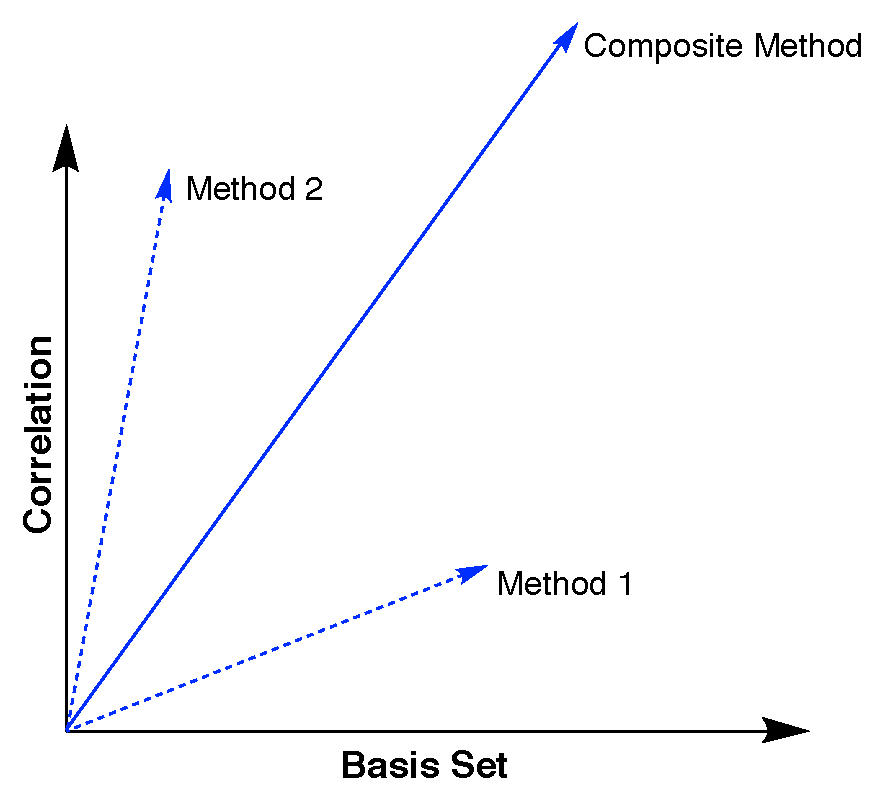
\includegraphics[height=20em]{figures/compositemethods.eps}
  \caption[Schematic representation of a quantum mechanical composite method.]{Schematic representation of a quantum mechanical composite method. The exact energy can only be achieved at the limits of an infinite basis set and complete correlation. Using a combination of Method 1 (low correlation/large basis set) and Method 2 (high correlation/small basis set), the Composite method approaches the exact energy.}
\label{fig:comp}
\end{figure}

\subsection{Density-functional theory}

Density-functional theory (DFT) is the most popular quantum chemical method applied to date. It relies on the two Hohenberg-Kohn theorems, the first of which states that there exists a unique electron density $\rho$ that defines the properties of a many-electron system. The second theorem defines an energy functional of the electron density and demonstrates that the correct ground state electron density minimises the energy functional through the variational theorem.\cite{Hohenberg1964,Koch2000} These theorems alone do not provide the solutions to the Schr{\"o}dinger equation.

It wasn't until the formulation of Kohn-Sham DFT\cite{Kohn1965} that the theory began gaining ground as a useful quantum theory. Kohn-Sham DFT scales formally with $N^3$ number of electrons\cite{Cramer2004} which is better than HF by a factor of $N$. In addition, DFT is a complete theory like FCI;\@ however, there is no straightforward way to determine the correct functionals of the electron density as the exact form of the functionals is unknown. Nonetheless, the drive for the development of the correct density-functional has been one of the main endeavours in quantum chemistry in the last two decades.

The framework behind conventional DFT is built into the description of the full energy functional $E$:

\begin{equation}
  E[\rho] = T_{ni}[\rho] + V_{ne}[\rho] + V_{ee}[\rho] + \Delta T[\rho] + \Delta V_{ee}[\rho]
\label{eq:DFT}
\end{equation}

\noindent where $T_{ni}$ is the kinetic energy of non-interacting electrons, $V_{ne}$ is the potential of nuclear-electron interactions, and $V_{ee}$ is the classical electron-electron repulsion. The last two terms are collectively referred to as the exchange-correlation (XC) functionals, where $\Delta T$ is the dynamical correlation term, and $\Delta V_{ee}$ is the non-classical correction to electron-electron repulsion. All the functionals, except the XC functionals have an exact form. It is therefore the XC functionals in which there is currently empiricism.

The ultimate goal in describing XC functionals is to find the ``correct'' XF functional which gives the exact energy of a system from the electron denisty. At this point, this must be done using approximations, for which there are several degrees of complexity. These approaches follow a hierarchical scheme, commonly referred to as the ``Jacob's ladder'' of DFT.\cite{Perdew2005} The first rung represents the simplest approximation which is known as local-density approximations (LDAs), which approximate the exchange-correlation density at a given point by the electron density at that same point. The form of these functionals is:

\begin{equation}
  E_{XC}^{LDA} = \int \rho (\mathbf{r}) \varepsilon_{XC} (\rho(\mathbf{r})) \mathrm{d}r
\end{equation}

\noindent where $\varepsilon_{XC}(\rho(\mathbf{r}))$ is the exchange-correlation energy per particle (energy density) of a uniform electron gas of density $\rho(\mathbf{r})$. This approximation is overly simple and applies only when the electron density if constant at all points, and are thus not generally applied in chemical problems. Nonetheless, LDA based approaches are commonly employed in solid state physics.

The second rung on the ladder corresponds to generalised-gradient approximation (GGA) based functionals, which are still amongst some of the most popular density-functionals. GGAs depend on both the electron density and the gradient of the electron density at a point:

\begin{equation}
  E_{XC}^{GGA} = \int \rho(\mathbf{r}) \varepsilon_{XC}^{GGA}(\rho(\mathbf{r}), \nabla \rho(\mathbf{r})) \mathrm{d}r
\end{equation}

\noindent where, $\varepsilon(\rho(\mathbf{r}), \nabla \rho(\mathbf{r})) \mathrm{d}r$ is the energy density associated with a given GGA.\@ GGA functionals provide a substantial improvement over LDAs, and most are constructed so that they correct the LDA energy:

\begin{equation}
  \varepsilon_{XC}^{GGA}(\rho(\mathbf{r}), \nabla \rho(\mathbf{r})) = \varepsilon_{XC}^{LDA}(\rho(\mathbf{r})) \mathrm{d}r + \Delta \varepsilon_{XC}\left( \frac{\nabla \rho(\mathbf{r})}{\rho^{4/3}({\mathbf{r}})}\right)
\end{equation}

A step above GGAs on the third rung of the ladder are meta-GGAs, which depend on the electron density, as well as the first derivative of electron density at a point, and the kinetic-energy density, $\tau(\mathbf{r})$, defined as:

\begin{equation}
  \tau(\mathbf{r}) = \sum_i^{occupied} \frac{1}{2}|\nabla \chi_i(\mathbf{r})|^2
\end{equation}

\noindent where $\chi_i(\mathbf{r})$ are the self-consistently determined Kohn-Sham orbitals. Meta-GGAs improve upon the accuracy of GGAs at a comparable cost.\cite{Cramer2004}

The XC functionals described up to this point (LDAs, GGAs, meta-GGAs) depend only on the electron density and derivatives of the electron density. The fourth and fifth rungs of the ladder improve upon the prior functionals by inclusion of terms dependent on additional properties. While this approach improves upon the accuracy of these functionals, it comes with an increase in computational cost. On the fourth rung sit functionals which depend to some percentage on the HF exact exchange. When the ratio of HF exchange is fixed, these functionals are termed hybrid functionals. Alternatively, functionals are said to be range-separated corrected if a different amount of exact-exchange to describe long and short-range behaviours. In the cases of hybrid and range-separated functionals, the added computational cost comes from the calculation of the HF exact exchange.

Alternatively, one can describe the fourth rung functionals as the depending upon the properties of the occupied molecular orbitals. The fifth rung then, is said to depend on the properties of unoccupied molecular orbitals. These functionals are typically referred to as double-hybrids, and incorporated correlation energy from a post-HF method, typically MP2.\cite{Goerigk2014} Double-hybrid DFT methods are once again more accurate than the lower rung methods, however, calculating the MP2 correlation energy is considerably more computationally demanding than traditional DFT approaches. Therefore, double-hybrid DFT methods have not gained popularity in the literature.

There are many published XC functionals. Fortunately, there is a fairly standard system of nomenclature, such that density functionals are described as \emph{exchange functional}-\emph{correlation functional}. The most commonly used density functional is the  B3-LYP, which uses the 3-parameter hybrid exchange functional of Becke,\cite{Becke1993} and the correlation functional of Lee, Yang, and Parr.\cite{Lee1988} There are also standalone functionals which have built in exchange and correlation functionals. A common example of these are the Minnesota family of functionals from the Truhlar group.\cite{Zhao2006,Zhao2006a}

Aside from the problem of choosing density-functionals, solving DFT is computationally very similar to the HF method. Within Kohn-Sham (KS) DFT, we define a fictitious system of non-interacting electrons with the same electron density as the real system. This is achieved by the use of a Hamiltonian in which there is an effective local potential, $V_s(\mathbf{r})$:

\begin{equation}
  \hat{H}_s = -\frac{1}{2}\sum_i^N\nabla_i^2 | \sum_i^N V_S(\mathbf{r}_i)
\end{equation}

\noindent The ground state wave function of this non-interacting Hamiltonian is represented by a single Slater determinant with spin orbitals ($\chi$), completely analogous to the HF problem. These spin orbitals, referred to as \emph{Kohn-Sham orbitals} are determined by

\begin{equation}
  \hat{h}_i^{KS} \chi_i = \varepsilon_i \chi_i
  \label{eq:kohnsham}
\end{equation}

\noindent where the one-electron Kohn-Sham operator $\hat{h}^{KS}$ is defined as

\begin{equation}
  \hat{h}_i^{KS} = -\frac{1}{2}\nabla^2 + V_s(\mathbf{r})
  \label{eq:ksoperator}
\end{equation}

It is crucial to realise that this procedure does not give us the exact energy of a system, but rather is used to determine an electron density which represents our real system. The connection between this fictitious system comes from the chose of the effective potential such that the density of our real system is a result of summing over the squared moduli of the KS orbitals:

\begin{equation}
  \rho(\mathbf{r}) = \sum_i | \chi_i |^2
\end{equation}

Once again in analogy to HF theory, on applies the variational principle to minimise the total energy functional in Equation~\ref{eq:DFT} with respect to $\chi$. The effective potential which variationally minimises the energy is given by\cite{Parr1995}

\begin{equation}
\begin{split}
  V_s(\mathbf{r}) &= \frac{\delta J[\rho]}{\rho(\mathbf{r})} + \frac{\delta E_{XC}[\rho]}{\delta \rho(\mathbf{r})} + \sum_A^M \frac{Z_A}{r_{iA}} \\
  &= \int\frac{\rho(\mathbf{r}_2)}{r_{12}} + V_{XC} + \sum_A^M \frac{Z_A}{r_{iA}}
\end{split}
\end{equation}

\noindent where the first term describes the Coulombic potential between two electrons, the last term is the potential between the electron and each nucleus. The middle term is once again the unknown XC potential. The electron density obtained from the fictitious system of non-interacting particles is finally used in Equation~\ref{eq:DFT} to find the total energy of the system. Since $V_s(\mathbf{r})$ depends on the electron density, these equation must be solvent iteratively, as with HF theory. Note however, that if the exact form of $E_{XC}[\rho]$ was known, this method would give the exact ground state electron density of the system, and thus the exact energy.

\subsubsection{Challenges for density-functional theory methods}

Pure DFT has low computational cost and potentially good accuracy, hence its popularity as a quantum chemical treatment. However, there are several problems which common DFT methods experience that lead to erroneous results in many cases.\cite{Cohen2012} It is well established that traditional DFT methods completely fail at describing non-covalent interactions.\cite{DiLabio2016} This shortcoming leads to poor descriptions of chemistry beyond equilibrium geometries, including transition states. Fortunately, there are several methods which can correct for this problem, commonly through the addition an energy correction term $E_{disp}$ to the DFT energy $E_{DFT}$, as

\begin{equation}
  E_{tot} = E_{DFT} + E_{disp}
\end{equation}

\noindent It is common to employ the empirical D3 pair-wise correction of Grimme,\cite{Grimme2010} paired with of the Becke-Johnson damping functions,\cite{Johnson2006} denoted as D3(BJ). This correction works by calculating the dispersion interactions between all pairs of atoms $A$ and $B$ separated by distance $R_{AB}$, with the following equation:

\begin{equation}
  E_{disp} - \sum_{A>B} \frac{C_6^{AB}}{R_{AB}^6} f_6(R_{AB}) + s_8
  \frac{C_8^{AB}}{R_{AB}^8} f_8(R_{AB})
\end{equation}

\noindent where $C_6$ and $C_8$ are dispersion coefficients, $s_8$ is an empirically determined scaling parameter, and $f_n$ are the damping functions which limit the range of dispersion correction, avoiding near singularities at small $R_{AB}$. Another approach to correcting for dispersion is to add parameters directly to the functional, as is the case in the Minnesota functionals.\cite{Zhao2006,Zhao2006} Both of these empirical corrections have the benefit of adding negligible computational time, but must be parametrised for each DFT method with which they are employed.

Another striking issue with DFT is the unphysical ability of an electron to interact with itself, termed \emph{self-interaction error}. This is most obvious in what is known as \emph{delocalisation error}, which is a result of many-electrons interacting with themselves, or many-electron self-interaction error. In HF theory, self-interaction error is exactly cancelled, thus DFT methods which have a high portion of HF exchange in their formulation are able to account for this issue. Consider for a moment a one electron system: there should be exactly zero electron correlation. In terms of the energy functionals shown in Equation~\ref{eq:DFT}, the electronic repulsion term $V_{ee}[\rho]$ should cancel exactly with the XC term ($V_{ee}[\rho] = -E_{XC}[\rho]$).\cite{Cramer2004} Unfortunately, all pure DFT methods fail to reproduce this expected behaviour. An obvious manifestation of delocalisation error is the incorrect treatment of charge-transfer in intramolecular interactions,\cite{MoriSanchez2008,OterodelaRoza2014} as well as in transition state complexes. Even for the simplest HAT reaction \ch{H2 + H^. -> H^. + H2}, the calculated barrier height is underestimated by 8--9 \kcalmol using a GGA functional.\cite{Csonka1998} Charge-transfer occurs when a fraction of an electron is transferred between molecular entities. Specifically, charge-transfer is mistreated at longer ranges, thus either high percentage exact exchange hybrid functionals, or range-separated functionals are suggested for systems in which charge-transfer may occur.

As is the case for most experimental methods, identifying the correct theoretical methods requires the careful consideration of the problem at hand. Choosing a DFT based method requires calibration, however, once a method has been tested and is known to provide reasonably accurate results, DFT methods have the ability to help understand chemical problem with relatively low computational costs.

\section{Applying theory to chemical problems}

\subsection{Geometry optimisation}

All QM methods depend parametrically on the geometry of a molecular system. That is the electronic energy of a system depends on the positions of the nuclei. While the wave functions can describe any arbitrary geometry, we are typically only interested in certain geometries of a molecule. These geometries of interest are normally stationary states along a the potential energy surface (PES) of a system, that is, points where the gradient of energy with respect to nuclear coordinates is zero. Therefore, we perform \emph{geometry optimisation} calculations to determine these points.

Molecular systems have complex PESs. For a non-linear molecule, the nuclear PES has 3$N$-6 dimensions, where $N$ is the number of nuclei present.\cite{Heidrich1991} In geometry optimisation, we seek the local minima (reactants, products, or intermediates) and local maxima (TS complexes). Consider only local minima for a moment. Often complex molecules have more than one possible conformation, and each conformation represents a different local minimum along the PES.\@ It is therefore important to ensure the correct conformation, typically the lowest energy structure (global minimum), is used when approaching chemical problems.

In order to efficiently perform geometry optimisation, numerical analysis techniques are employed. All geometry optimisation methods follow the same general framework.\cite{Hratchian2005} First, energy and necessary derivatives are computed from an initial geometry. Second, the geometry is modified to step towards the nearest stationary state. And last, some test is performed to determine if the new geometry is near enough to the stationary state along the PES.\@ The most efficient method to do this is the \emph{Newton method}, in which the energy is expanded in a Taylor series (truncated at the second order point) about the current point, $\mathbf{x}_0$:

\begin{equation}
  E(\mathbf{x}) = E_0 + \mathbf{g}_0\Delta\mathbf{x} + \frac{1}{2}\Delta\mathbf{x}\mathbf{H}_0\Delta \mathbf{x}
\end{equation}

\noindent where $E_0$, $\mathbf{g}_0$, and $\mathbf{H}_0$ are the energy, gradient (Jacobian), and second derivative (Hessian) at point $\mathbf{x}_0$, and $\Delta \mathbf{x} = x_i - x_0$. The aim of the Newton method is to minimise the gradient of the Taylor expansion, $\mathbf{g(x)}$, such that

\begin{equation}
  \mathbf{g(x)} = \mathbf{g}_0 + \mathbf{H}_0 \Delta \mathbf{x}
\end{equation}

\noindent Solving for $\Delta \mathbf{x}$ gives the so-called Newton step that leads to minimisation:

\begin{equation}
  \Delta \mathbf{x} = -\mathbf{H}^{-1}_0\mathbf{g}_0
\end{equation}

The analytic computation of the Hessian is very expensive, especially for large systems. Therefore, to simply the problem at the beginning of geometry optimisation, the Hessian matrix is approximated and updated at each step in the optimisation, using clever algorithms.\cite{Hratchian2005} This is called the \emph{quasi-Newton method}, and is the default optimisation routine in the Gaussian\cite{Frisch2009} quantum chemistry package, as well as many other quantum chemistry packages.

Some additional caution must be taken in optimising molecular structures. Normal algorithms which optimise structures stop when the gradient of energy is sufficiently close to zero; however, often PES can be flat or very shallow in regions and structures that are not fully optimised can be obtained. To avoid this, geometries are always subject to molecular vibration analysis.

\subsection{Molecular vibrations}

The computation of molecular vibrations can be performed simply given a set of molecular coordinates.\cite{Wilson1980} Assuming a non-linear molecule, we start with 3$N$-6 internal coordinates which are non-coupled (orthogonal). We then apply the \emph{harmonic approximation}, in which we assume each normal mode follows Hooke's Law

\begin{equation}
  F = kx
\end{equation}


\noindent where $F$ is the force, $k$ is the force constant, and $x$ is the displacement along one normal mode's coordinates. This approximation assumes the PES along the normal mode is parabolic, which in general is not true, but is a good approximation near the minima. Deviations from this approximation are known as \emph{anharmonicity}. In practise, however, at normal temperatures ($\sim$ 298K) the harmonic approximation is sufficient to describe molecular vibrations as displacements are assumed to be small.

Typically to obtain molecular frequencies, one computes the mass-weighted Hessian matrix elements $F_{ij}$

\begin{equation}
  F_{ij} = \frac{1}{\sqrt{m_i m_j}} \mathbf{H}_{ij}
\end{equation}

\noindent where the partial derivatives of internal coordinates $x_i$ of the potential energy $U$ are taken for 3$N$ atoms with mass $m$. One then seeks to diagonalise this $3N\times3N$ matrix to obtain eigenvalues $\lambda_i$, which describe the force constant of each normal mode. The harmonic frequencies $\nu_i$ are then obtained by

\begin{equation}
  \nu_i = \frac{\sqrt{\lambda_i}}{2\pi}
\end{equation}

\noindent and the lowest 6 modes are then discarded to account for 3$N$-6 normal modes. These lowest energy modes generally correspond the internal rotations, and thus must be discarded to correctly obtain thermochemical corrections.

From these frequencies, the \emph{zero-point vibrational energy} (ZPE, $E_{ZPE}$) is calculated:

\begin{equation}
  E_{ZPE} = \sum_{i=1}^{3N-6} \frac{h\nu_i}{2}
\end{equation}

\noindent The ZPE is an important quantum correction to the classical potential, giving the electronic potential energy

\begin{equation}
U = E_{elec} + E_{ZPE}
\end{equation}

\noindent where $E_{elec}$ is the QM electronic energy.

If a normal mode describes a non-minimum along the PES, the energy gradient will be negative (imaginary) instead of positive. Only energy maxima or saddle-points (TS structures) should have a single imaginary mode. Therefore, if a non-TS molecular structure calculation yields one or more imaginary modes, the geometry optimisation has yielded a structure which is not at minimum on the PES.\@ In this situation additional steps must be taken to find a corrected structure.

\subsection{Thermochemistry}

Up until this point we have been viewing molecules from a microscopic perspective; however, this is not useful for describing properties of bulk systems. Fortunately, fundamental statistical thermodynamics can be used to approximately describe a system in bulk.\cite{McQuarrie1999,McQuarrie2000} We approximate our system as an ensemble of non-interacting particles: the ideal gas. Within statistical thermodynamics, the fundamental starting point is the partition function $Q$,\cite{note4} from which all thermodynamic properties can be calculated. For our ensemble, the molecular partition function is

\begin{equation}
  Q = \sum_J e^{\varepsilon_j/k_B T}
\end{equation}

\noindent where a Boltzmann distribution of $j$ energy states $\varepsilon$ is taken at temperature $T$, and $k_B$ is the Boltzmann constant. All calculations herein are defined under conditions of temperature $T$ = 298.15 K and pressure $P$ = 1 atm.

Normally, the molecular partition function is decomposed into contributions from translational, vibrational, rotational, and electronic motion:

\begin{equation}
  Q = q_{trans}q_{vib}q_{rot}q_{elec}
\end{equation}

\noindent The equation describing the translational partition function
$q_{trans}$ is

\begin{equation}
  q_{trans} = \left( \frac{2\pi m k_B T}{h^2} \right)^{3/2} \frac{k_B T}{P}
\end{equation}

\noindent where $m$ is the mass of the molecule, $h$ is Planck's constants.

The vibrational partition function $q_{vib}$ depends on the contributions of each of $K$ vibrational modes. Only the $3N-6$ (or $3N-5$ for linear molecules) real vibrational modes of a molecule are considered, and imaginary frequencies are ignored. Therefore, for molecules which posses an imaginary frequency this thermodynamic analysis is invalid. TS complexes do posses a single imaginary frequency which is ignored, as it is assumed to not contribute to the overall vibrational partition function as no formal bond is said to be formed in the acceptor-donor system. Each vibrational mode has a characteristic vibrational electronic temperature, $\Theta_{\nu,K} = h\nu/k_B$, and the partition function is

\begin{equation}
  q_{vib} = \prod_K \frac{e^{-\Theta_{\nu,K}/2T}}{1 - e^{-\Theta_{\nu,K}/T}}
\end{equation}

The rotational partition function depends on the geometry of a system. For a single molecule $q_{rot}$=1. For a linear molecule, the rotational partition function is

\begin{equation}
  q_{rot} = \frac{1}{\sigma_r} \left(\frac{T}{\Theta_r}\right)
\end{equation}

\noindent where $\sigma_r$ is the symmetry number for rotation which depends on the molecular symmetry, and $\Theta_r = h^2/8\pi^2Ik_B$. $I$ is the moment of inertia. Finally, for a non-linear polyatomic molecule, the rotational partition function is

\begin{equation}
  q_{rot} = \frac{\sqrt{\pi}}{\sigma_r}\left(\frac{T^{3/2}}{\sqrt{\Theta_{r,x}\Theta_{r,y}\Theta_{r,z}}}\right)
\end{equation}

\noindent where $\Theta_{r,x}, \Theta_{r,y}$, and $\Theta_{r,z}$ describe contributions of the moment of inertia in each of the x, y, and z-planes.

Finally, we make an important assumption that electronic contributions are assumed to exist in only the ground state, as excited states are generally safely assumed to be much larger than $k_B T$ in energy. The full electronic partition function is

\begin{equation}
  q_{elec} = \sum_{i=0} \omega_i e^{-\epsilon_i/k_B T}
\end{equation}

\noindent where $\omega$ is the degeneracy of an energy level with energy $\epsilon$. Applying our assumption, and by setting the ground state energy $\epsilon_0=0$, our problem simplifies dramatically, such that $q_{elec} = \omega_0$, which is simply the spin multiplicity of the molecule.

We now have all the information needed to calculate the thermodynamic quantities we are interested in. In chemistry we are concerned with the Gibbs free energy $G$, which is defined by the entropy $S$ and enthalpy $H$ as

\begin{equation}
  G = H - TS
\end{equation}

\noindent From each of the partition functions, the entropy of a system with $N$ moles, $S_{tot} = S_{trans} + S_{vib } +S_{rot} + S_{elec}$, is calculated using the relation

\begin{equation}
  S = Nk_B + Nk_B\ln\left( \frac{Q}{N} \right) + Nk_B T \left( \frac{\partial
      \ln Q}{\partial T} \right)_V
\end{equation}

\noindent Similarly, the internal energy of a system, $E_{int,tot} = E_{int,trans} + E_{int,vib} + E_{int,rot} + E_{int,elec}$, is given by the relation

\begin{equation}
  E_{int} = Nk_B T^2\left( \frac{\partial \ln Q}{\partial T} \right)_V
\end{equation}

\noindent Finally, the enthalpy is obtained from

\begin{equation}
  H_{tot} = E_{int,tot} + k_B T
\end{equation}

Using very simple statistical thermodynamic arguments, the properties of a bulk system are easily computed. It is important to emphasise that these results are for particles in the gas phase, thus additional steps must be taken if one desires to compare results to experiments performed in solvent.

\subsection{Modelling solvent}

It is in principle possible to include solvent molecules explicitly in QM calculations: this is in practise, extremely cost prohibitive. In order to approximate the important contributions of solvation, so-called \emph{implicit continuum solvent models} are generally employed.\cite{Mennucci2007,Cramer2004} Mathematically, one describes this as

\begin{equation}
  \hat{H}^{tot}(\mathbf{r}_m) = \hat{H}^{mol}(\mathbf{r}_m) + \hat{V}^{mol+sol}(\mathbf{r}_m)
\end{equation}

\noindent where a perturbation $\hat{V}^{mol+sol}$ dependent only on the coordinates of the solute ($\mathbf{r}_m$; thus implicit) is applied to the Hamiltonian of the solute. The perturbation term is composed of interaction operators which contribute to the net free energy:

\begin{equation}
G_{solv} = G_{cavity} + G_{electrostatic} + G_{dispersion} + G_{repulsion} +
G_{solv~kinetic}
\end{equation}

\noindent where the total solvation free energy $G_{solv}$ contains terms from: the formation of a solvation cavity $G_{cavity}$, the electrostatic interactions between solvent and solute $G_{electrostatic}$, the dispersion interactions between solvent and solute $G_{dispersion}$, the QM exchange repulsion between solvent and solute $G_{repulsion}$, and the movement of solvent molecules $G_{solv~kinetic}$.

A widely used model for solvation comes from the Truhlar group, and is known as SMD.\cite{Marenich2009} The main parameter in implicit solvent models is the solvent dielectric constant ($\varepsilon$) with contributions from surface tension and the solvent-solute interface. SMD also includes terms which depend on the electron density of the solute.  While many other implicit solvent models require the use of the same QM method as they were parametrised,\cite{Ho2010} SMD is a \emph{universal} model which was parametrised using several QM methods. Therefore, it does not require the use of a specific QM method and can be applied broadly in both single point energy and geometry optimisation calculations.

\subsection{Rate constants and transition state theory}

In the discussion of chemical kinetics, the rate ($r$) of a bimolecular reaction

\begin{equation}
  \ch{$a$ A + $b$ B <=> $c$ C + $d$ D}
  \label{eq:a}
\end{equation}

\noindent is determined by the \emph{rate law}, which can generally be described as

\begin{equation}
  r = \frac{d \text{C}}{dt} =\frac{d \text{D}}{dt} = k[A]^a [B]^b
\end{equation}

\noindent where $k$ is the rate constant, $t$ is time, $A, B, C$, and $D$ are chemical species with stoichiometric coefficients $a, b, c$, and $d$, and $k$ is the rate constant. Computational chemistry is in general, not useful for determining rate laws: this must be done experimentally. Where computational studies can be useful, is in determining reaction mechanisms, and how the reaction barrier height can be altered. In doing so, we focus entirely on $k$.

Most chemists are intimately familiar with the phenomenological \emph{Arrhenius equation}

\begin{equation}
  k_{Arr} = Ae^{-E_a/RT}
\label{eq:arrhenius}
\end{equation}

\noindent where $A$ is a constant, $R$ is the gas constant, and $E_a$ is the \emph{activation energy}, which is an experimental measure of the reaction barrier height. This equation dates back to the 1880s, when Arrhenius noticed that the reactions depended more heavily on temperature than was intuitive, and thus introduced the $A$ constant, known often as the Arrhenius pre-factor.\cite{McQuarrie1997} The Arrhenius pre-factor is an empirical measure of how factors other than kinetic energy affect the rate constant. From the perspective of theory, Equation~\ref{eq:arrhenius} has little meaning as the parameters are empirical. Thus, to study rate constants theoretically we must turn to \emph{transition state theory}.

\subsubsection{Transition state theory}

The study of transition state theory (TST) originates in the 1930s, and was developed primarily by Eyring.\cite{McQuarrie1997,Steinfeld1998} In TST we focus on the TS complex, which is defined as a transient species which exists at the top of the energy barrier of a reaction. If we consider the same reaction in Equation~\ref{eq:a}, and set all the coefficients to 1, then TST states the reaction proceeds in two steps, the first of which includes a quasi-equilibrium between the reactants and TS complex

\begin{equation}
  \ch{A + B <=>AB$^\ddagger$ <=> C + D}
  \label{eq:tst}
\end{equation}

\noindent with an equilibrium constant ($K_c^{\ddagger}$) expression

\begin{equation}
  K_c^{\ddagger} = \frac{[\ch{AB}^\ddagger]/c^0}{[\ch{A}]/c^0[\ch{B}]/c^0}
\label{eq:K}
\end{equation}

\noindent where $c^0$ is the standard-state concentration (normally taken to be 1 M).

\begin{figure}[htb]
    \centering
    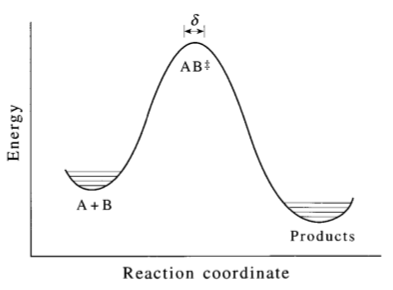
\includegraphics[width=0.6\textwidth]{figures/TST-PES.png}
    \caption[A reaction coordinate diagram for a generic reaction.]{A reaction coordinate diagram for the reaction of Equation~\ref{eq:tst}. The TS complex is defined to exist in the small region $\delta$ above the reaction barrier.}
\label{fig:tst-pes}
\end{figure}

In TST, we define the TS complex to exist throughout a small region of width $\delta$ above the reaction barrier (\ref{fig:tst-pes}). From the second step of the reaction in Equation~\ref{eq:tst}, we can define a reaction rate dependent on the concentration $[\ch{AB}^\ddagger]$ and $v_c$, a factor which defines the frequency with which the complexes proceed over the barrier:

\begin{equation}
  r = v_c [\ch{AB}^\ddagger]
\end{equation}

From Equations~\ref{eq:a} and~\ref{eq:tst}, we now have two equivalent expressions for the reaction rate, which allows us to derive the following

\begin{equation}
  r = k[\ch{A}][\ch{B}] = v_c [\ch{AB}^\ddagger]
\end{equation}

\noindent and solving Equation~\ref{eq:K} for $[\ch{AB}^\ddagger]$ results in


\begin{equation}
  r = v_c\frac{[\ch{A}][\ch{B}]K_c^\ddagger}{c^0}
\end{equation}

\noindent or

\begin{equation}
  k = \frac{v_c K_c^\ddagger}{c^0}
\label{eq:b}
\end{equation}

We must now invoke the statistical thermodynamics to make sense of Equation~\ref{eq:b}. We can rewrite the equilibrium expression $K_c^\ddagger$ in terms of partition functions of each molecular species:

\begin{equation}
    K_c^{\ddagger} = \frac{[\ch{AB}^\ddagger]/c^0}{[\ch{A}]/c^0[\ch{B}]/c^0}
    = \frac{(q^\ddagger/V)c^0}{(q_A/V)(q_b/V)}
\label{eq:c}
\end{equation}

\noindent where $V$ is the volume, and $q_A$, $q_B$, and $q^\ddagger$ are the partition functions of A, B, and AB$^\ddagger$, respectively.

Since we have defined the reaction to be occurring with one degree of freedom, the translational partition function $q_{trans}$ can be defined as

\begin{equation}
  q_{trans} = \frac{\sqrt{2\pi m^\ddagger k_B T}}{h}\delta
\end{equation}

\noindent where $m^\ddagger$ is the mass of the TS complex. The partion function of the TS complex can be written as the product $q^\ddagger = q_{trans}q_{int}^\ddagger$, where the second term accounts for all remaining degrees of freedom of the TS complex. We can use this and rewrite Equations~\ref{eq:c} and~\ref{eq:b} as

\begin{equation}
  K_c^{\ddagger} =  \frac{\sqrt{2\pi m^\ddagger k_B T}}{h}\delta\frac{(q_{int}^\ddagger/V)c^0}{(q_A/V)(q_b/V)}
\end{equation}

\noindent and

\begin{equation}
 k = v_c \frac{\sqrt{2\pi m^\ddagger
     k_B T}}{hc^0}\delta\frac{(q_{int}^\ddagger/V)c^0}{(q_A/V)(q_b/V)}
\label{eq:d}
\end{equation}

We are now left with the two terms $v_c$ and $\delta$ which are ill-defined. However, the product of these two terms is the average speed at which the TS complex crosses the barrier, $\langle u_{TS} \rangle = v_c\delta$. A Maxwell-Boltzmann distribution is used to calculate the value of $\langle u_{TS} \rangle$:

\begin{equation}
  \langle u_{TS} \rangle = \left( \frac{m^\ddagger}{2\pi k_B T} \right)^{1/2}
  \int_0^\infty u e^{-m^\ddagger u^2/2k_B T}du = \left( \frac{m^\ddagger}{2\pi
      k_B T m^\ddagger} \right)^{1/2}
\label{eq:e}
\end{equation}

\noindent Substituting Equation \ref{eq:e} into Equation~\ref{eq:d} for $v_c\delta$ yields

\begin{equation}
  k =
  \frac{\sqrt{k_B T}}{hc^0}\frac{(q_{int}^\ddagger/V)c^0}{(q_A/V)(q_b/V)} = \frac{k_B T}{hc^0}K_c^\ddagger
\label{eq:f}
\end{equation}

Now, define the standard Gibbs free energy of activation ($\Delta ^\ddagger G^0$) to be the change in Gibbs free energy in going from reactants to TS.\@ The thermodynamical expression is

\begin{equation}
  \Delta ^\ddagger G^0 = -RT \ln K_c^\ddagger
\end{equation}

\noindent which can be substituted into Equation~\ref{eq:f}

\begin{equation}
  k = \frac{k_B T}{hc^0} e^{-\Delta^\ddagger G^0/RT}
\label{eq:g}
\end{equation}

The standard Gibbs free energy of activation can be expressed in terms of enthalpy and entropy as

\begin{equation}
  \Delta^\ddagger G^0 = \Delta^\ddagger H^0 - T \Delta^\ddagger S^0
\end{equation}

\noindent which, upon substitution gives the equation

\begin{equation}
  k = \frac{k_B T}{hc^0} e^{-\Delta^\ddagger S^0/R} e^{-\Delta^\ddagger H^0/RT}
\label{eq:M}
\end{equation}

At this point, we can draw a direct comparison to the Arrhenius equation (Equation~\ref{eq:arrhenius}) by expressing $E_a$ in terms of $\Delta^\ddagger H^0$ and $A$ in terms of $\Delta^\ddagger S^0$.  We must differentiate the natural logarithm of Equation~\ref{eq:f}, as well as Equation~\ref{eq:arrhenius} (assuming that $A$ is independent of temperature):

\begin{equation}
  \frac{d \ln k}{dT} = \frac{1}{T} + \frac{d \ln K_c^\ddagger}{dT}
  \label{eq:h}
\end{equation}

\begin{equation}
  \frac{d \ln k_{Arr}}{dT} = \frac{E_a}{RT^2}
  \label{eq:i}
\end{equation}

\noindent Next, we use the fact that $d \ln K_c / dT = \Delta U^0/RT^2$ for an ideal gas, then Equation \ref{eq:h}  becomes

\begin{equation}
  \frac{d \ln k}{dT} = \frac{1}{T} + \frac{\Delta ^\ddagger U^0}{RT^2}
  \label{eq:j}
\end{equation}

\noindent Additionally, $\Delta ^\ddagger H^0 = \Delta ^\ddagger U^0 + RT \Delta^\ddagger n$ ($\Delta^\ddagger n = 1$), as so Equation~\ref{eq:j} can be rewritten as

\begin{equation}
  \frac{d \ln k}{dT} = \frac{\Delta ^\ddagger H^0 + 2RT}{RT^2}
  \label{eq:k}
\end{equation}

\noindent Therefore, by comparison of Equation~\ref{eq:k} and \ref{eq:i}, we get

\begin{equation}
  E_a = \Delta^\ddagger H^0 + 2RT
  \label{eq:Ea-vs-dH}
\end{equation}

\noindent which then converts Equation~\ref{eq:M} into the form

\begin{equation}
  k = \frac{e^2k_B T}{hc^0}e^{\Delta^\ddagger S^0/R}e^{-E_a/RT}
\end{equation}

Therefore, a statistical thermodynamical picture of the Arrhenius equation arises from TST, and the Arrhenius pre-factor $A$ can be expressed as

\begin{equation}
  A = \frac{e^2k_B T}{hc^0}e^{\Delta^\ddagger S^0/R}
\label{eq:afactor}
\end{equation}

In practise, we use the form of Equation~\ref{eq:g} to compute the rate constant of a reaction, which we shall denote as $k_{TST}$. The conventional TST makes an assumption that the reaction coordinate is static along the lowest energy pathway. This can be corrected by the use of \emph{variational transition state theory}.\cite{Truhlar1984} We shall not consider variational TST in this work, as with careful application, conventional TST does a remarkably good job at accounting for the magnitude and temperature dependence of a wide range of reactions.\cite{Steinfeld1998} Additionally, if one makes corrections for \emph{QM tunnelling}, conventional TST can easily give a more complete description of the rate constant.

\subsubsection{Quantum mechanical tunnelling}

Atoms are quantum mechanical particles, and are thus subject to the strange probabilistic behaviours observed at the microscopic level. QM tunnelling refers to the ability of particles to penetrate the reaction barrier, rather than surmounting it classically (\ref{fig:tunnelling}). While all reactions are subject to QM tunnelling, we will show that due to the low mass of the hydrogen atom, QM tunnelling can play a significant role in HAT reactions.

\begin{figure}[htb]
  \centering
  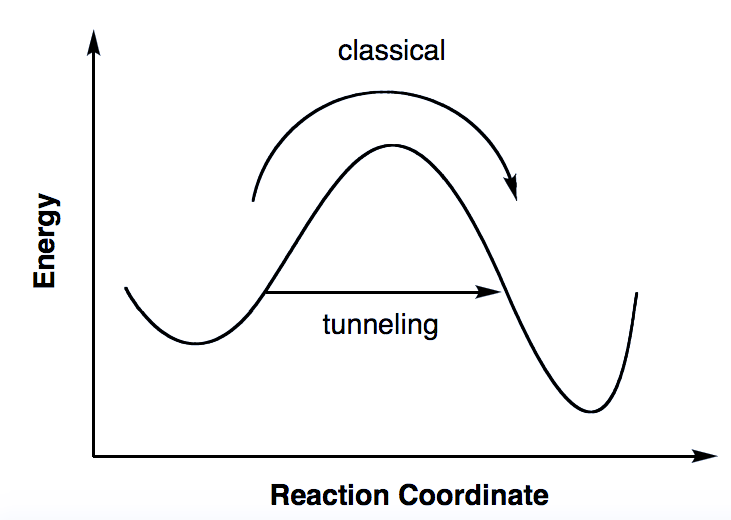
\includegraphics[width=0.5\textwidth]{figures/tunnelling-1}
  \caption{Quantum mechanical tunnelling occurs when a particle penetrates a
    reaction barrier, rather than surmounting it. Figure adapted from Reference~\citenum{McMahon2003}.}
\label{fig:tunnelling}
\end{figure}


In order to determine the effects of scattering, one must find transmission coefficients ($\kappa$) by solving the Schr{\"o}dinger equation.\cite{Griffiths2016} This is done by approximating the reaction barrier with an analytical potential, thus simplifying the problem mathematically. The earliest model potentials were introduced by Bell, who used a parabolic function to approximate the reaction barrier.\cite{Bell1980} To obtain $\kappa$, and thus the observed rate constant ($k_{obs}$), the following equations were used:

\begin{align}
  k_{obs} &= \kappa A e^{-E_a/RT}  \\
\kappa &= \frac{e^\alpha}{\beta-\alpha} \left(\beta e^{-\alpha} - \alpha
  e^{-\beta} \right) \\
  \alpha &= E_a/RT \\
  \beta &= \frac{2a\pi^2(2mE_a)^{1/2}}{h}
\end{align}

\noindent where the Arrhenius equation was used to estimate the rate constant, $m$ is the mass of the tunnelling particle, and $2a$ is the width of the barrier. Since the equation is dependent on the mass of the particle, tunnelling occurs more often when lighter particles are involved. As a consequence, tunnelling is more common in HAT reactions than other atom transfer reactions. Also, the height and width of the barrier are important factors in determining the contributions to tunnelling: reactions with small barriers have low tunnelling contributions; narrow barriers result in higher tunnelling contributions.

The Bell model is a poor representation of an actual reaction barrier. One which is a much better approximation is the \emph{Eckart potential}.\cite{Johnston1962} The form of this potential is

\begin{align}
  V &= -\frac{Ay}{1-y} - \frac{By}{1-y^2} \\
  y &= -e^{2\pi x/L}
\end{align}

\noindent where $x$ is the variable along the reaction coordinate and $L$ is called the characteristic length. If $A=0$ the potential becomes a symmetric function, further simplifying the problem; however, most reactions do not have a symmetric potential. $A$, $B$ and $L$ are related to the change in barrier height in the forward and reverse direction, $\Delta V_1$ and $\Delta V_2$, respectively:

\begin{align}
  A &= \Delta V_1 - \Delta V_2 \\
  B &= ((\Delta V_1)^{1/2} + (\Delta V_2)^{1/2})^2 \\
 \frac{L}{2\pi} &= (-\frac{2}{F^*})^{1/2} [\frac{1}{(\Delta V_1)^{1/2}} +
      \frac{1}{(\Delta V_2)^{1/2}}]^{-1}
\end{align}

\noindent where $F^* = d^2V/dx^2$ evaluated at the maximum of the potential. In this formulation, $V$ is a placeholder energy. Note that if a reaction is endoergic, tunnelling does not occur. Alternatively, one says tunnelling only occurs in exoergic or energy-neutral reactions.

The solutions to the Schr{\"o}dinger equation for the Eckart potential are analytical, thus that transmission coefficient $\kappa$ can easily be computed using standard numerical techniques. These tunnelling corrections will be applied, where applicable as

\begin{equation}
  k_{calc} = \kappa k_{TST} = \kappa
\frac{k_B T}{hc^0}e^{-\Delta^\ddagger G^0}
\end{equation}
